\documentclass{beamer}
\usetheme{Madrid}
% \usetheme{default}
% \usecolortheme{beaver}
\usepackage{graphicx}
\graphicspath{ {pics} }
\usepackage{amsmath}
\usepackage{amssymb}
\usefonttheme[onlymath]{serif}

%Information to be included in the title page:
\title{Algebra}
\author{Nithin}
\institute{Maveric Systems}
\date{\today}

\begin{document}
\frame{\titlepage}

\begin{frame}{Origins of Algebra}
    \begin{itemize}
      \item \textbf{Mesopotamia \& Egypt (c. 2000–1600 BCE)}
        \begin{itemize}
          \item Early problem-solving (linear/quadratic equations) in word problems
          \item No formal symbols, but systematic procedures
        \end{itemize}
  
      \item \textbf{Greek Era (c. 600 BCE–300 CE)}
        \begin{itemize}
          \item Geometric methods for solving equations (Euclid, Apollonius)
          \item Diophantus introduced proto-symbolic notation
        \end{itemize}
  
      \item \textbf{Islamic Golden Age (8th–12th Century)}
        \begin{itemize}
          \item Al-Khwarizmi’s work \emph{Al-jabr} $\rightarrow$ term “Algebra”
          \item Systematic solutions for linear and quadratic equations
        \end{itemize}
  
      \item \textbf{Transmission to Europe (12th–17th Century)}
        \begin{itemize}
          \item Latin translations influenced Fibonacci, others
          \item Viète, Descartes established modern symbolic notation \& analytic geometry
        \end{itemize}
  
      \item \textbf{Modern Algebra (19th–20th Century)}
        \begin{itemize}
          \item Emergence of abstract algebra (groups, rings, fields)
          \item Galois, Abel, and others formalized algebraic structures
        \end{itemize}
    \end{itemize}
  \end{frame}

  \begin{frame}{What is Algebra?}
    Algebra is a branch of mathematics that deals with numbers, variables, and their relationships. Key concepts include:
    
    \begin{itemize}
        \item \textbf{Variables}: Symbols (like \( x \), \( y \)) representing unknown or changing values.
        \item \textbf{Expressions}: Combinations of variables, numbers, and operations. E.g., \( 2x + 3 \).
        \item \textbf{Equations}: Mathematical statements that express equality, e.g., \( 2x + 3 = 7 \).
        \item \textbf{Solving Equations}: Finding values for variables that make an equation true.
        \item \textbf{Polynomials}: Expressions like \( 3x^2 + 2x - 5 \) involving variables raised to powers.
        \item \textbf{Functions}: Describes a relationship between variables, e.g., \( y = 2x + 1 \).
    \end{itemize}
\end{frame}


  \begin{frame}{Integers}
    \begin{itemize}
        \item The set of integers is denoted by \(\mathbb{Z}\).
        \item Integers include:
        \[
          \ldots, -3, -2, -1, 0, 1, 2, 3, \ldots
        \]
        \item Formally, \(\mathbb{Z} = \{\dots, -2, -1, 0, 1, 2, \dots\}\).
        \item Common properties:
        \begin{itemize}
            \item \(\mathbb{Z}\) is infinite and unbounded in both the negative and positive directions.
            \item Closed under addition, subtraction, and multiplication:
                \[
                  \forall a, b \in \mathbb{Z}, \quad
                  a \pm b \in \mathbb{Z}, \quad
                  a \cdot b \in \mathbb{Z}.
                \]
        \end{itemize}
        \item The quotient of any two integers is not necessarily an integer. So we need to extend arithmetic to \textbf{rational numbers}
    \end{itemize}
\end{frame}

% Slide: Rational Numbers
\begin{frame}{Rational Numbers}
    \begin{itemize}
        \item The set of rational numbers is denoted by \(\mathbb{Q}\).
        \item Definition:
        \[
          \mathbb{Q} = \left\{ \frac{p}{q} \,\middle|\,
            p \in \mathbb{Z}, \; q \in \mathbb{Z}, \; q \neq 0
          \right\}.
        \]
        \item Every integer is also a rational number (e.g., \(5 = \frac{5}{1}\)).
        \item Examples:
        \[
          \frac{1}{2}, \quad -\frac{3}{4}, \quad 0, \quad 7, \quad \frac{11}{5}, \ldots
        \]
        \item Properties:
        \begin{itemize}
            \item Closed under addition, subtraction, multiplication, and division (except division by zero).
            \item Densely packed on the number line: between any two rationals, there is another rational.
        \end{itemize}
    \end{itemize}
\end{frame}

\begin{frame}
    \frametitle{Interesting Facts}
    \begin{itemize} 
        \item Why division by zero is prohibited ?
        \begin{itemize}
            \item Division is inverse of multiplication in the sense  
            \[  
            \frac{m}{n} \cdot n = m
            \]
        \item if \( n=0 \) and \( m = 1\), we get \(\frac{1}{0} \cdot 0 = 1\) which is nonsensical as any number multiplied by zero is zero
        \end{itemize}
        \item Rational numbers suffice for all actual physical measurements like weight, height and length
        \item But Geometry, Algebra and Calculus force us to consider \textbf{real numbers}
    \end{itemize}
\end{frame}

\begin{frame}
    \frametitle{A Real Number Line}
    \begin{figure}[h]    
        \begin{minipage}[b]{0.8\textwidth}
        \centering
        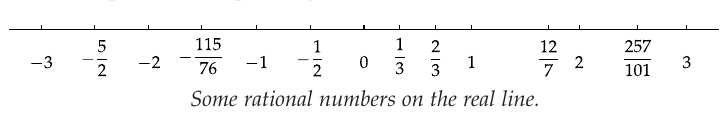
\includegraphics[scale=0.35]{real-line.png}
    \end{minipage}
\end{figure}
\begin{itemize}
    \item if \( n\) is a positive integer then \( \frac{1}{n}\) is to the right of 0 by the length obtained by dividing the segment from \( 1 to 0\) in to \( n \) segments of equal length
\end{itemize}
\end{frame}

\begin{frame}
    \frametitle{Is every Real Number a Rational}
    \begin{figure}[h]    
        \begin{minipage}[b]{0.8\textwidth}
        \centering
        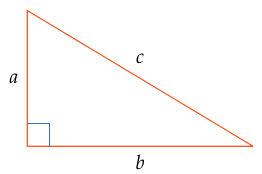
\includegraphics[scale=0.35]{irrational-geometry.png}
        \end{minipage}
    \end{figure}
    \begin{itemize}
        \item \( c^{2} = a^{2} + b^{2} \). If \( a = 1, b = 1\) then \(c^{2} = 2 \). Then what rational number is \( c \)
        \item By trial and error, \( c = \left( \frac{99}{70} \right)^{2}  = \frac{9801}{4900}\) where the numerator just misses twice the denominator by 1. But this is not 2 but close to 2. Another number is \( \left( \frac{9369319}{6625109} \right)^{2} = 1.999999999999977\) , but not 2
        \item Greeks proved that it is impossible to find any rational number whose square is 2
    \end{itemize} 
\end{frame}

\begin{frame}
    \frametitle{Proof: No rational number has a square equal to 2}
    Let m and n are two integers
    \[ 
        \left( \frac{m}{n} \right)^{2} = 2  
    \]
    By canceling any common factors, m and n are reduces to its lowest terms 

    \[
         m^{2} = 2n^{2}
    \]

    this makes \(m^{2}\) even, hence \(m\) is an even. (The square of even is even and odd is odd). So \(m = 2k\) for some integer \(k\)

    Substituting \(m = 2k\) in the equation gives, \(4k^{2} = 2n^{2} \), which results in 
    \[
        2k^{2} = n^{2}
    \]
    which means \( n^{2}\) is even and therefore \(n \) is even
    \\
    \(\frac{m}{n} \) has common factors which contradicts the earlier assumption
\end{frame}

\begin{frame}
    \frametitle{Irrational Number}

    \begin{block}{Irrational Number}
        A real number that is not rational is \textbf{irrational number}
    \end{block}
    \begin{itemize}
        \item \( \sqrt(2)\)
        \item \(3+\sqrt(2)\)
        \item \(8\sqrt(2)\)
    \end{itemize}
\end{frame}

\section{Algebra of real numbers}

\begin{frame}{Properties of Real Numbers}
  \begin{itemize}
      \item \textbf{Commutative Properties}
      \begin{itemize}
          \item Addition: $a + b = b + a$
          \item Multiplication: $a \cdot b = b \cdot a$
      \end{itemize}
      \vspace{5pt}

      \item \textbf{Associative Properties}
      \begin{itemize}
          \item Addition: $(a + b) + c = a + (b + c)$
          \item Multiplication: $(a \cdot b) \cdot c = a \cdot (b \cdot c)$
      \end{itemize}
      \vspace{5pt}
      \item \textbf{Distributive Property}
      \begin{itemize}
          \item $a \cdot (b + c) = (a \cdot b) + (a \cdot c)$
      \end{itemize}
      \vspace{5pt}
      \item \textbf{Identity Elements}
      \begin{itemize}
          \item Additive Identity: $a + 0 = a$
          \item Multiplicative Identity: $a \cdot 1 = a$
      \end{itemize}
      \vspace{5pt}
      \item \textbf{Inverse Elements}
      \begin{itemize}
          \item Additive Inverse: $a + (-a) = 0$
          \item Multiplicative Inverse (if $a \neq 0$): $a \cdot \frac{1}{a} = 1$
      \end{itemize}
    \end{itemize}
    \end{frame}
    \begin{frame}{Properties of Real Numbers}
    \begin{itemize}
      \vspace{5pt}
      \item \textbf{Closure Property}
      \begin{itemize}
          \item Real numbers are closed under addition, subtraction, multiplication, and division (except division by zero).
      \end{itemize}
  \end{itemize}
  \end{frame}
\subsection{Inequalities,Intervals and Absolute Value}
\begin{frame}
  \frametitle{Inequalities}
  \begin{block}{Transitivity}
    \begin{itemize}
        \item If $a < b$ and $b < c$, then $a < c$
      \end{itemize}
  \end{block}

  \begin{block}{Multiplication}
    Suppose $a < b$
    \begin{itemize}
      \item If $c > 0$, then $ac < bc$
      \item If $c <  0$, then $ ac > bc$
    \end{itemize}
  \end{block}
\end{frame} 

\begin{frame}
  \frametitle{Exercise }
  Find all number \( x \) such that 
  \[\frac{x-8}{x-4} < 3 \] 
Our first step  is to multiply by \(x-4\)
Here there are two conditions:
\begin{enumerate}
  \item \( x-4 > 0 \) 
  \[ x -8 < 3(x-4)  \implies x-8 < 3x-12 \implies 2x > 4  \implies x > 2\]
  But our initial assumption is \(x-4 > 0 \implies x > 4 \). As \( 4 > 2 \), original inequality holds if \( x > 4\)
\end{enumerate} 
\end{frame}

\begin{frame}
  \frametitle{Exercise Conti.}
\begin{enumerate}
  \setcounter{enumi}{1}
  \item \( x-4 < 0 \) 
  \[ x-8 > 3(x-4) \implies  x < 2 \] 
  Initial assumption is \( x<4 \). As \( 2 < 4\), inequality holds for \( x < 2 \)
\end{enumerate}

The original inequality holds true for \[x < 2 ,  x > 4 \]   
or 
\[  (-\infty, 2) \cup (4,\infty) \]

\end{frame}

\begin{frame}
  \frametitle{Inequalities}
  \begin{block}{Additive Inverse}
    If \( a < b \) then \( -a > -b \)
    Direction of inequalities has to be reversed when taking additive inverses on both sides 
  \end{block}
  \begin{block}{Multiplicative Inverse}
    If \( a < b \) 
    \begin{itemize}
      \item If \(a > 0, b > 0\), then \(\frac{1}{a} > \frac{1}{b} \)
      \item If \(a < 0 < b\), then \(\frac{1}{a} < \frac{1}{b} \)
    \end{itemize} 
  \end{block}

\end{frame}

\begin{frame}{What is a Set?}
  \begin{block}{Definition}
      A \textbf{set} is a well-defined collection of distinct objects, called \textbf{elements} or \textbf{members} of the set.
  \end{block}

  \vspace{10pt}

  \textbf{Representation of a Set:}
  \begin{itemize}
      \item \textbf{Roster Form:} List elements inside curly braces:
      \[
      A = \{1, 2, 3, 4\}
      \]
      \item \textbf{Set-Builder Notation:} Describe properties of elements:
      \[
      A = \{x \mid x \text{ is a positive integer less than 5}\}
      \]
  \end{itemize}

  \vspace{10pt}

  \begin{block}{Membership}
      \begin{itemize}
          \item If \(x\) belongs to \(A\), write \(x \in A\).
          \item If \(x\) does not belong to \(A\), write \(x \notin A\).
      \end{itemize}
  \end{block}
\end{frame}

\begin{frame}{Types of Sets}
  \begin{block}{Types of Sets}
      \begin{itemize}
          \item \textbf{Finite Set:} A set with a countable number of elements. \\
          Example: \(A = \{1, 2, 3, 4\}\)
          
          \item \textbf{Infinite Set:} A set with an uncountable or infinite number of elements. \\
          Example: \(\mathbb{N} = \{1, 2, 3, \dots\}\)

          \item \textbf{Empty/Null Set:} A set with no elements, denoted as \(\emptyset\) or \(\{\}\).

          \item \textbf{Subset:} \(A \subseteq B\) if every element of \(A\) is in \(B\).

          \item \textbf{Universal Set:} A set containing all objects under consideration, usually denoted by \(U\).

          \item \textbf{Power Set:} The set of all subsets of \(A\), denoted as \(P(A)\). \\
          Example: If \(A = \{1, 2\}\), then \(P(A) = \{\emptyset, \{1\}, \{2\}, \{1, 2\}\}\).
      \end{itemize}
  \end{block}
\end{frame}

\begin{frame}{Set Operations}
  \begin{block}{Union (\(\cup\))}
      Combines elements of two sets:
      \[
      A \cup B = \{x \mid x \in A \text{ or } x \in B\}
      \]
  \end{block}

  \begin{block}{Intersection (\(\cap\))}
      Elements common to both sets:
      \[
      A \cap B = \{x \mid x \in A \text{ and } x \in B\}
      \]
  \end{block}

  \begin{block}{Difference (\(A - B\))}
      Elements in \(A\) but not in \(B\):
      \[
      A - B = \{x \mid x \in A \text{ and } x \notin B\}
      \]
  \end{block}

\end{frame}



\begin{frame}{Set Operations}
  \begin{block}{Complement (\(A^c\))}
    Elements not in the set \(A\):
    \[
    A^c = \{x \mid x \notin A\}
    \]
\end{block}

  \begin{block}{Examples}
      \begin{itemize}
          \item The set of natural numbers: \(\mathbb{N} = \{1, 2, 3, \dots\}\).
          \item The set of integers: \(\mathbb{Z} = \{\dots, -3, -2, -1, 0, 1, 2, 3, \dots\}\).
          \item The set of even numbers: \(\{2, 4, 6, \dots\}\).
      \end{itemize}
  \end{block}
\end{frame} 



\begin{frame}{What is an Interval?}
  \begin{block}{Definition}
      An \textbf{interval} is a set of real numbers that includes all the numbers between two given endpoints.
  \end{block}
  \vspace{10pt}
  Intervals describe ranges of values on the real number line and are widely used in mathematics.
\end{frame}

% Slide 3: Types of Intervals
\begin{frame}{Types of Intervals}
  \begin{itemize}
      \item \textbf{Closed Interval (\([a, b]\))}: Includes both endpoints \(a\) and \(b\).
      \[
      [a, b] = \{x \in \mathbb{R} \mid a \leq x \leq b\}
      \]
      Example: \([2, 5] = \{x \mid 2 \leq x \leq 5\}\).
      \vspace{5pt}

      \item \textbf{Open Interval (\((a, b)\))}: Excludes both endpoints \(a\) and \(b\).
      \[
      (a, b) = \{x \in \mathbb{R} \mid a < x < b\}
      \]
      Example: \((2, 5) = \{x \mid 2 < x < 5\}\).
  \end{itemize}
\end{frame}

% Slide 4: Half-Open Intervals
\begin{frame}{Half-Open or Half-Closed Intervals}
  \begin{itemize}
      \item \textbf{Left-Closed, Right-Open (\([a, b)\))}:
      \[
      [a, b) = \{x \in \mathbb{R} \mid a \leq x < b\}
      \]
      Example: \([2, 5) = \{x \mid 2 \leq x < 5\}\).
      \vspace{5pt}

      \item \textbf{Left-Open, Right-Closed (\((a, b]\))}:
      \[
      (a, b] = \{x \in \mathbb{R} \mid a < x \leq b\}
      \]
      Example: \((2, 5] = \{x \mid 2 < x \leq 5\}\).
  \end{itemize}
\end{frame}

% Slide 5: Infinite Intervals
\begin{frame}{Infinite Intervals}
  \begin{itemize}
      \item \((a, \infty)\): All numbers greater than \(a\).
      \[
      (a, \infty) = \{x \in \mathbb{R} \mid x > a\}
      \]
      Example: \((3, \infty)\) includes all numbers greater than 3.

      \item \((-\infty, b)\): All numbers less than \(b\).
      \[
      (-\infty, b) = \{x \in \mathbb{R} \mid x < b\}
      \]
      Example: \((-\infty, 4)\) includes all numbers less than 4.

      \item \((-\infty, \infty)\): The entire real number line.
      \[
      (-\infty, \infty) = \mathbb{R}
      \]
  \end{itemize}
\end{frame}

% Slide 6: Summary Table
\begin{frame}{Summary of Interval Types}
  \begin{tabular}{|c|c|c|}
      \hline
      \textbf{Type} & \textbf{Interval Notation} & \textbf{Description} \\
      \hline
      Closed         & \([a, b]\)      & Includes both endpoints \(a, b\) \\
      Open           & \((a, b)\)      & Excludes both endpoints \(a, b\) \\
      Half-Open Left & \([a, b)\)      & Includes \(a\), excludes \(b\) \\
      Half-Open Right & \((a, b]\)     & Excludes \(a\), includes \(b\) \\
      Infinite Left  & \((-\infty, b)\)& All \(x < b\) \\
      Infinite Right & \((a, \infty)\) & All \(x > a\) \\
      Entire Line    & \((-\infty, \infty)\) & All real numbers \\
      \hline
  \end{tabular}
\end{frame}




\begin{frame}{What is Absolute Value?}
  \begin{block}{Definition}
      The \textbf{absolute value} of a number is its distance from zero on the number line, regardless of direction. It is always non-negative.
  \end{block}

  \vspace{10pt}

  For a real number \(x\), the absolute value, denoted as \(|x|\), is defined as:
  \[
  |x| =
  \begin{cases} 
  x, & \text{if } x \geq 0, \\
  -x, & \text{if } x < 0.
  \end{cases}
  \]
\end{frame}

% Slide 3: Examples
\begin{frame}{Examples of Absolute Value}
  \begin{itemize}
      \item \(|3| = 3\) \quad (because \(3 \geq 0\))
      \item \(|-5| = -(-5) = 5\) \quad (because \(-5 < 0\))
      \item \(|0| = 0\) \quad (because \(0\) is neither positive nor negative)
  \end{itemize}
\end{frame}

% Slide 4: Properties of Absolute Value
\begin{frame}{Properties of Absolute Value}
  \begin{itemize}
      \item \textbf{Non-Negativity:} \(|x| \geq 0\) for all \(x\).
      \item \textbf{Identity Property:} \(|x| = 0 \quad \text{if and only if } x = 0.\)
      \item \textbf{Multiplicative Property:} \(|x \cdot y| = |x| \cdot |y|\).
      \item \textbf{Triangle Inequality:} \(|x + y| \leq |x| + |y|\).
      \item \textbf{Distance Interpretation:} \(|x - y|\) represents the distance between \(x\) and \(y\).
  \end{itemize}
\end{frame}


\begin{frame}
  \frametitle{Exercises}
Ball bearings need to have extremely accurate sizes to work correctly. The ideal diameter of a particular ball bearing is 0.8 cm, but a ball bearing is declared
acceptable if the error in the diameter size is less than 0.001 cm. Write the inequality for acceptance criteria
\vspace{0.5cm}

Solution: \pause
The ball bearings are acceptable if  diameter \( d \) is 
\[ | d-0.8| \leq 0.001 \]

\end{frame}

\begin{frame}
  \frametitle{Exercises}
  Find all numbers \(t \) such that \( |3t-4| = 10\)

  \vspace{5pt} 

  Solution : \pause  
  \[ 3t -4  = 10  \; or \; 3t-4 = -10  \implies t = \frac{14}{3}, t = -2 \]
\end{frame} 

\begin{frame}
  \frametitle{Exercise}
  Find all numbers \(x\) such that \[ \left| \frac{3x-5}{x-1} \right|< 2 \]

  \vspace{5pt}



\end{frame}



\end{document}